
\section{Aplikacja mobilna}
Implementację aplikacji mobilnej rozpocząłem od kreatora, w którym wybrałem opcję pojedynczego Activity. Na początku zaimplementowałem odpowiednie algorytmy skanujące sieci bezprzewodowe w zasięgu. W kolejnym kroku dodałem obsługę urządzenia GPS. Następnie stworzyłem tabelę w bazie danych aplikacji mobilnej z odpowiednią strukturą do przechowywania zebranych obserwacji sieci bezprzewodowych. Na koniec zaimplementowałem prezentację geolokalizacji uzyskanej z aplikacji internetowe oraz możliwość eksportu zebranych obserwacji lokalizacji sieci bezprzewodowych.

\subsection{Uprawnienia na Android}

Począwszy od Androida 6.0 (poziom API 23), użytkownicy przyznają uprawnienia do aplikacji podczas uruchamiania aplikacji, a nie podczas instalowania aplikacji. To podejście usprawnia proces instalacji, ponieważ użytkownik nie musi przyznawać uprawnień podczas instalowania lub aktualizacji. Daje to również użytkownikowi większą kontrolę nad funkcjonalnością aplikacji; Na przykład użytkownik może się zdecydować, czy udostępnić kamerę dostęp do aparatu, ale nie do lokalizacji urządzenia. Dodatkowo użytkownik może cofnąć uprawnienia w dowolnym momencie, przechodząc do ekranu \textit{Ustawienia aplikacji}.\cite{NewPermissionsModelInAndroid60}

Nowy system uprawnień wymaga dodatkowej uwagi twórców aplikacji mobilnych. Zanim

\subsection{Skanowanie sieci bezprzewodowych}
Klasycznym przykładem tego, jak Android został zaprojektowany, jest własnie skanowanie sieci bezprzewodowych. Aby uzyskać obiekty klasy ScanResults. Po pierwsze, musimy uzyskać instancję programu WifiManager. Następnie dziedzicząc po klasie BroadcastReceiver zaimplementować metodę, która dostanie powiadomienie o zakończeniu przetwarzania. Taki asynchroniczny odbiornik — WifiScanReceiver — rejestrujemy z parametrem WifiManager.SCAN_RESULTS_AVAILABLE_ACTION i wreszcie rozpocząć skanowanie przez metodę startScan() na instancji WifiManager.

\begin{minted}{java}
wifi_manager = (WifiManager) getApplicationContext().getSystemService(Context.WIFI_SERVICE);
wifi_scan_reciever = new WifiScanReceiver();
registerReceiver(wifi_scan_reciever, new IntentFilter(WifiManager.SCAN_RESULTS_AVAILABLE_ACTION));
wifi_manager.startScan();
\end{minted}

I tu niespodzianka, bo w Androidzie nie mamy możliwości zaparametryzowania, że chcemy uzyskiwać wyniki o zeskanowanych sieciach w sposób ciągły. Musimy więc w naszym WifiScanReceiver zlecić ponowne skanowanie zaraz po otrzymaniu wyniku ostatniego skanowania. Tutaj jeszcze dodałem małe sprawdzenie, czy mamy aktualne współrzędne geograficzne do zapisania lokalizacji.

\begin{minted}{java}
private class WifiScanReceiver extends BroadcastReceiver {
        public void onReceive(Context context, Intent intent) {
            wifi_manager.startScan();
            if( last_location != null && ( (1000*10) > Calendar.getInstance().getTime().getTime() - last_location.getTime())){
                List<ScanResult> wifiScanList = wifi_manager.getScanResults();
                for (ScanResult wifi : wifiScanList) {
                    if( wifi.SSID.contains("_nomap") || wifi.SSID.contains("_optout") ){
                        wifiScanList.remove(wifi);
                    }
                }

                JSONArray array = new JSONArray();
                if (wifiScanList.size() == 0) {
                    wifis.add(getString(R.string.no_networks));
                } else {
                    ActiveAndroid.beginTransaction();
                    try {
                        for (ScanResult wifi : wifiScanList) {
                            WifiObservation wifiObservation = new WifiObservation(wifi, last_location);
                            array.put(wifiObservation.toJson());
                            wifiObservation.save();
                        }
                        ActiveAndroid.setTransactionSuccessful();
                    } finally {
                        ActiveAndroid.endTransaction();
                    }
                    runJavascript("geolocateByWifis("+array.toString()+")");
                }

            }
        }
    }
\end{minted}
W powyższym kodzie źródłowym widzimy usuwanie wyników zeskanowanych sieci z określonymi dopiskami. Wiąże się to z faktem, że Google zaproponowało dopisywanie do końca nazwy sieci \_nomap (z ang. nie mapuj), aby ich rozwiązania nie zbierały informacji o lokalizacji danych sieci bezprzewodowych.\cite{GoogleNomap} Dodatkowego zamieszania dorzuciła firma Microsoft, gdzie dla swoich rozwiązań zaproponowali \_optout (z ang. wypisz mnie).\cite{MicrosoftOptout}

\subsubsection{Problem z określeniem kierunku sygnału}
Nie jest możliwym stwierdzenie, z jakiego kierunku przyszedł sygnał sieci bezprzewodowej. Powoduje to, że zbieranie informacji o lokalizacjach sieci bezprzewodowych jest skazane na dużą niedokładność. Konkretniej spowoduje to umiejscowienie wszystkich sieci bezprzewodowych na pozycji telefonu dla algorytmów bardzo prymitywnych Np. na środku ulicy lub na chodniku. Bardzo dobrze to widać na /refs{fig:poor-scan-result}

\begin{figure}[h!]
  \centering
    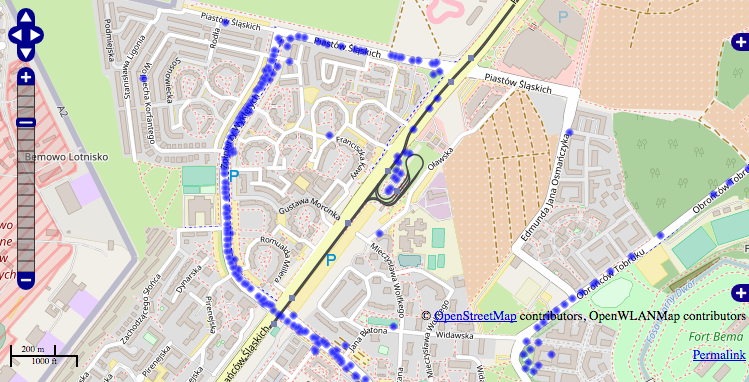
\includegraphics[width=10cm]{images/poor-scan-result}
  \caption{Prezentacja lokalizacji sieci bezprzewodowych na mapie - algorytm primitywny}
  \label{fig:poor-scan-result}
\end{figure}

Rozwiązaniem lepsze, ale droższe byłoby użycie kilku urządzeń, najlepiej z antenami kierunkowymi, dzięki czemu moglibyśmy stwierdzić czy stacja bazowa znajduje się po lewej stronie ulicy, czy po prawej na podstawie siły sygnału.
Dzięki technologii MIMO można określić, z którego kierunku przyszedł sygnał na jednym urządzeniu. Ze względu na denormalizację obserwacji sieci bezprzewodowych jesteśmy w stanie estymować kierunek, z którego przyszedł sygnał o ile mamy kilka zarejestrowanych skanów z różnymi siłami i lokalizacjami.


\subsection{Określanie lokalizacji urządzenia}
Do obsługi lokalizacji urządzenia poprzez GPS wykorzystałem bibliotekę — SmartLocation. Użycie prostego interfejsu biblioteki zaoszczędziło dużo czasu, który musiałbym poświęcić na zapoznawanie się z dokumentacją klas i interfejsów dotyczących nawigacji w Androidzie.

\begin{minted}{java}
public void startGpsListener(){
    SmartLocation.with(this).location().config(LocationParams.NAVIGATION).continuous().start(gps_location_listener);
}
private class GpsLocationListener implements OnLocationUpdatedListener {
    @Override
    public void onLocationUpdated(Location location) {
        last_location = location;
    }
}
\end{minted}

Sam proces uzyskania informacji o lokalizacji urządzenia jest asynchroniczny. Aby zniwelować efekt asynchroniczności, utworzyłem lokalną zmienną w ramach widoku, do której zapisuję ostatnią otrzymaną pozycję z SmartLocation. Do uzyskania najdokładniejszej pozycji skorzystałem z funkcji trybu nawigacji (z ang. navigate) z parametrem pracy ciągłej (z ang. continious). Trzeba pamiętać, że takie ustawienie jest niekorzystne dla czasu pracy na baterii, ale gwarantuje to najświeższą informację o współrzędnych urządzenia.

\subsection{Baza danych}
Teraz gdy już mamy wyniki skanowania sieci bezprzewodowych i lokalizację urządzenia, to jesteśmy w stanie zapisać wyniki do bazy danych aplikacji mobilnej — aby potem przesłać do aplikacji internetowej — dla lepszej precyzji określania lokalizacji sieci bezprzewodowych, a tym samym użytkownika.

Wybrałem bibliotekę ActiveAndroid jako ORM ze względu na swoje podobieństwo do ActiveRecord ze świata języka programowania Ruby oraz ze względu na użycie bazy SQLite, która jest popularnym rozwiązaniem do przechowywania danych na Androidzie. Stosując się do dobrych praktych twórców tej biblioteki, umieściłem tworzenie obserwacji w transakcji:

\begin{minted}{java}
ActiveAndroid.beginTransaction();
try {
    for (ScanResult wifi : wifiScanList) {
        WifiObservation wifiObservation = new WifiObservation(wifi, last_location);
        wifiObservation.save();
    }
    ActiveAndroid.setTransactionSuccessful();
} finally {
    ActiveAndroid.endTransaction();
}
\end{minted}

Po raz kolejny podjąłem decyzję o denormalizacji danych. Dane takie będą zajmować więcej miejsca, ale umożliwią na dokładniejsze lokalizowanie miejsca, w którym jest umiejscowiony punkt dostępu. Wszystkie dane będą zapisane w pojedynczej tabeli.

\begin{table}
\caption{Kolumny i typy przechowywania danych wraz z ich znaczeniem}
\label{table:dbscheme}
\begin{tabular} { |l|l|p{7cm}|  }
\hline
Typ & Nazwa & Znaczenie (opcjonalne) \\
\hline
\hline
String & ssid & \\
\hline
String & bssid & \\
\hline
int & signal_level & Wykryty poziom sygnału w dBm, znany również jako RSSI.\cite{scanResultAndroidDocs} \\
\hline
String & capabilities & Opisuje schematy uwierzytelniania, zarządzania kluczami i szyfrowania obsługiwane przez punkt dostępu.\cite{scanResultAndroidDocs} \\
\hline
Date & observed_at & Data i czas o sieć została zeskanowana \\
\hline
int & channel_frequency & Częstotliwość zeskanowanej sieci \\
\hline
double & latitude & Szerokość geograficzna pozycji w której sieć zeskanowano \\
\hline
double & longitude & Wysokość geograficzna pozycji w której sieć zeskanowano \\
\hline
Date & geolocated_at & Data i czas otrzymania informacji o współrzędnych geograficznych urządzenia \\
\hline
float & geolocation_accuracy & Dokładność współrzędnych geograficznych pozycji w któ®ej sieć zeskanowano \\
\hline
boolean & is_exported & Informacja o tym czy sieć została wyeksportowana do aplikacji internetowej \\
\hline
\end{tabular}
\end{table}

Konstruktor klasy WifiObservation przyjmujący zeskanowaną sieć oraz ostatnią lokalizację zaimplementowałem następująco:
\begin{minted}{java}
public WifiObservation(ScanResult scanResult, Location location){
    super();
    this.ssid = scanResult.SSID;
    this.bssid = scanResult.BSSID;
    this.signal_level = scanResult.level;
    this.capabilities = scanResult.capabilities;
    this.channel_frequency = scanResult.frequency;

    this.observed_at = new Date();

    this.latitude = location.getLatitude();
    this.longitude = location.getLongitude();
    this.geolocated_at = new Date(location.getTime());
    this.geolocation_accuracy = location.getAccuracy();

    this.is_exported = false;
}
\end{minted}

\subsection{Prezentacja danych — mapa}

% dodałem flagę "android wake lock flag" żeby ekran się nie usypiał
% trzeba było włączyć CORS
